\lstset{
  basicstyle=\ttfamily,
  columns=fullflexible,
  frame=single,
  breaklines=true,
  showlines=true,
  postbreak=\mbox{\textcolor{red}{$\hookrightarrow$}\space},
}

\chapter{Analisis}
\label{chap:analisis}
Pengumpulan data dalam skripsi ini dilakukan dengan cara studi pustaka.

\section{Analisis BlueTape}
\label{sec:analisisbluetape}
\begin{figure}[H]
	\centering  
	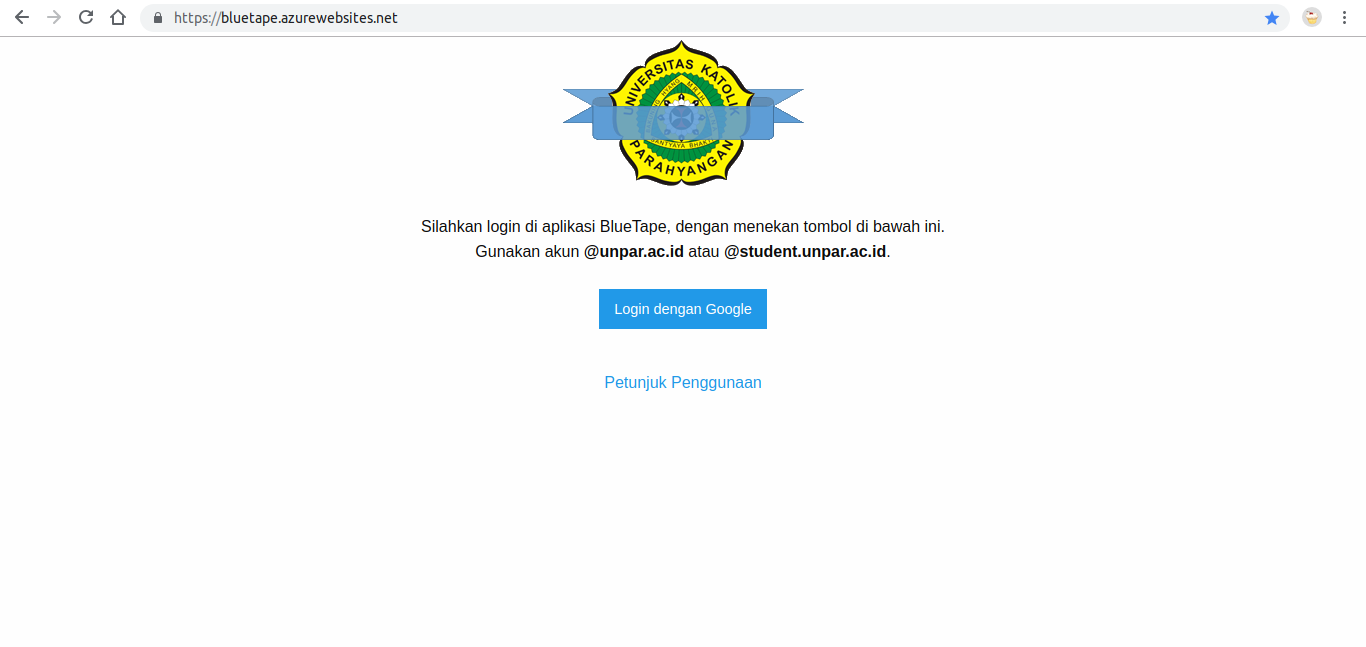
\includegraphics[width=\textwidth]{bluetape-login.png}  
	\caption[Tampilan utama BlueTape]{Tampilan utama BlueTape} 
	\label{fig:bluetape-login} 
\end{figure}

\textit{BlueTape} adalah perangkat lunak yang berfungsi untuk membantu urusan-urusan \textit{paper-based} di FTIS UNPAR menjadi \textit{paperless}. Pada saat skripsi ini dibuat, BlueTape dapat diakses melalui situs web \url{https://bluetape.azurewebsites.net/} (Gambar~\ref{fig:bluetape-login}). Perangkat lunak ini bersifat open source, sehingga kode program BlueTape bisa dipelajari, diubah, dan distribusi oleh siapapun untuk tujuan apapun. Kode program ini dapat diakses di \url{https://github.com/ftisunpar/BlueTape}. BlueTape memanfaatkan CodeIgniter (versi 3.1.4) dan ZURB Foundation.

Pola pengembangan yang dipakai BlueTape adalah MVC (Model-View-Controller). MVC (Model-View-Controller) adalah sebuah metode untuk membuat perangkat lunak menjadi tiga bagian : Model, View, dan Controller. Model adalah kelas yang merepresentasikan struktur data. View adalah informasi yang disajikan ke pengguna. Controller adalah penghubung antara Model, View, dan sumber daya lain yang dibutuhkan untuk mengolah HTTP request dan menghasilkan situs web.

\subsection{Aturan Konstribusi BlueTape}
Terdapat beberapa aturan apabila ingin berkonstribusi pada pengembangan BlueTape. Aturan-aturan tersebut tertera pada dokumen \texttt{CONTRIBUTING.md} (\url{https://github.com/ftisunpar/BlueTape/blob/master/CONTRIBUTING.md}).
\subsubsection{Pengelompokkan Module}
Perangkat lunak BlueTape dikelompokkan dalam module. Setiap module memiliki nama yang mengikuti aturan CamelCase. Jika beberapa module tergabung pada satu topik yang sama, topik tersebut harus digunakan sebagai kata pertama dalam penamaan module. Contohnya : apabila nama topik adalah \texttt{Transkrip}, maka contoh nama modulenya adalah \texttt{TranskripRequest} dan \texttt{TranskripManage}.

Penamaan dokumen pada controller, view, model, config file, nama tabel, dan migration script menggunakan nama module atau topik. Contoh penamaan :
\begin{itemize}
\item Controller: \texttt{controllers/TranskripRequest.php}, \texttt{controllers/TranskripManage.php}
\item View: \texttt{views/TranskripRequest/*.php}, \texttt{views/TranskripManage/*.php}
\item Model (opsional): \texttt{models/Transkrip/*\_model.php}
\item Config file (opsional): \texttt{config/Transkrip.php}
\item Nama tabel (opsional): \texttt{Transkrip}
\item Migration script (opsional): \texttt{migrations/20160222120000\_Transkrip\_initial.php}
\end{itemize} 

\subsubsection{Model}
Model dibuat hanya jika fungsi-fungsi di dalamnya digunakan lebih dari sekali. Apabila hanya digunakan sekali, letakkan fungsi pada controller.

\subsubsection{Library \texttt{bluetape}}
Library \texttt{bluetape} berisi fungsi-fungsi yang umum digunakan di BlueTape. Contoh : fungsi untuk konversi email ke NPM.

\subsubsection{Hak Akses}
Hak akses dan nama module diatur pada dokumen \texttt{config/modules.php}. Contoh :
\begin{lstlisting}
$config['module-names'] = array(
    'TranskripRequest' => 'Permohonan Cetak Transkrip',
    'TranskripManage' => 'Manajemen Cetak Transkrip'
);

$config['modules'] = array(
    'TranskripRequest' => array('root', 'mahasiswa.ftis'),
    'TranskripManage' => array('root', 'tu.ftis')
);

$config['roles'] = array(
    'root' => 'pascal@unpar\\.ac\\.id',
    'tu.ftis' => '(shao\\.wei)@unpar\\.ac\\.id',
    'mahasiswa.ftis' => '7[123]\\d{5}@student\\.unpar\\.ac\\.id'
);
\end{lstlisting}

Apabila diperlukan, kontributor boleh menambahkan role baru pada array config "roles". Setiap elemen array memetakan role dengan alamat email yang tergabung dalam role tersebut, dengan notasi regular expression.

\subsection{Autentikasi}
Setiap module wajib memeriksa hak akses sebekum ditampilkan. 
Hal tersebut dilakukan dengan cara memanfaatkan template berikut pada controller:
\begin{lstlisting}
<?php
defined('BASEPATH') OR exit('No direct script access allowed');
class NamaPage extends CI_Controller {

    public function __construct() {
        parent::__construct();
        try {
            $this->Auth_model->checkModuleAllowed(get_class());
        } catch (Exception $ex) {
            $this->session->set_flashdata('error', $ex->getMessage());
            header('Location: /');
        }
    }

    // ... implementasikan method-method Anda yang lain di sini...
}
\end{lstlisting}

\subsubsection{View}
Setiap view menggunakan template yang menampilkan nama module, menu navigasi, dan \textit{flash message} (jika diperlukan). Setiap view membutuhkan parameter \texttt{currentModule}, selain parameter-parameter lainnya. Jika ingin memanggil view dari controller, fungsi \texttt{get\_class()} dapat digunakan. Berikut adalah cara sederhana memanggil view :  
\begin{lstlisting}
$this->load->view('NamaPage/main', array('currentModule' => get_class()));
\end{lstlisting}

View memanfaatkan framework Zurb Foundation, dan berisi template menu utama serta flash message. Oleh karena itu, kode berikut digunakan untuk memulai membuat view :
\begin{lstlisting}
<?php
defined('BASEPATH') OR exit('No direct script access allowed');
?><!doctype html>
<html class="no-js" lang="en">
    <?php $this->load->view('templates/head_loggedin'); ?>
    <body>
        <?php $this->load->view('templates/topbar_loggedin'); ?>
        <?php $this->load->view('templates/flashmessage'); ?>

        <!-- Tulislah isi view Anda di sini. -->

        <script src="/public/foundation-6/js/vendor/jquery.min.js"></script>
        <script src="/public/foundation-6/js/vendor/what-input.min.js"></script>
        <script src="/public/foundation-6/js/foundation.min.js"></script>
        <script src="/public/foundation-6/js/app.js"></script>
    </body>
</html>
\end{lstlisting}

\subsection{Fitur - Fitur BlueTape}
Saat skripsi ini ditulis, BlueTape memiliki perangkat lunak BlueTape memiliki tiga layanan, yaitu Transkrip \textit{Request} / \textit{Manage}, Perubahan Kuliah \textit{Request} / \textit{Manage}, dan perekam jadwal dosen. Layanan Transkrip \textit{Request} / \textit{Manage} memberikan layanan untuk melakukan permohonan serta pencetakan transkrip mahasiswa. Layanan Perubahan Kuliah \textit{Request} / \textit{Manage} memberikan layanan untuk permohonan dan pencetakan perubahan jadwal kuliah oleh dosen. Layanan perekam jadwal dosen untuk merekam dan menampilkan jadwal dosen.

\subsubsection{Transkrip \textit{Request}}
\begin{figure}[H]
	\centering  
	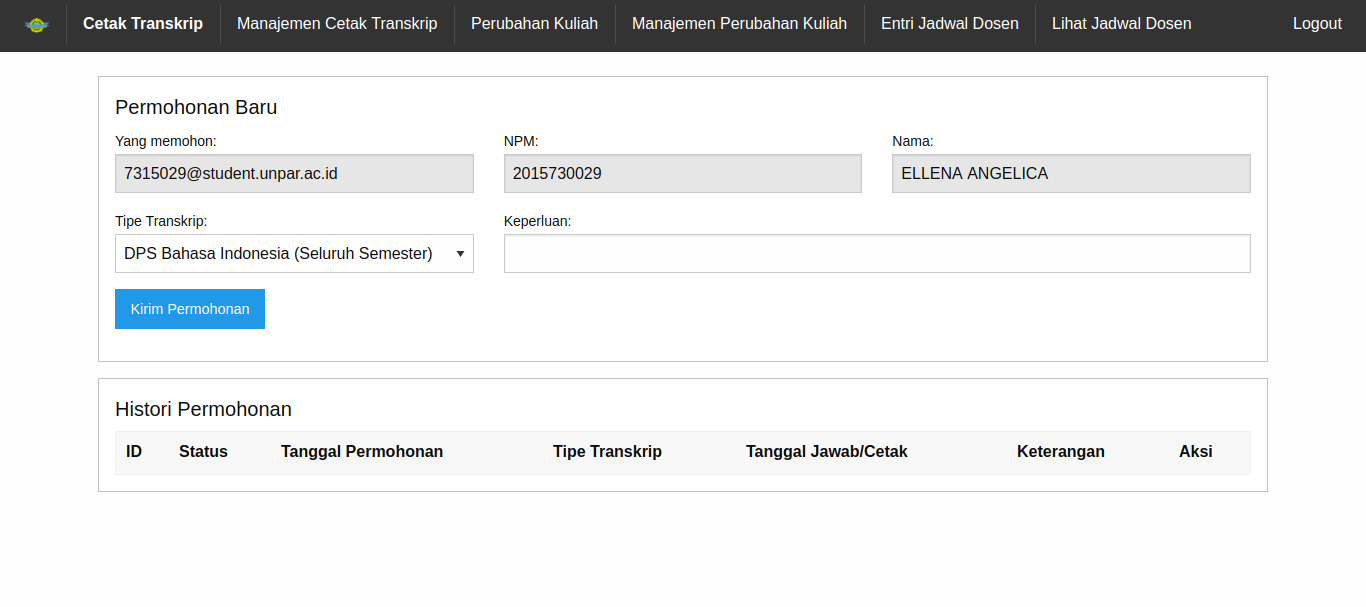
\includegraphics[width=\textwidth]{bluetape-cetak-transkrip.png}  
	\caption[Tampilan Cetak Transkrip]{Tampilan Cetak Transkrip} 
	\label{fig:bluetape-cetak-transkrip} 
\end{figure}

\begin{figure}[H]
	\centering  
	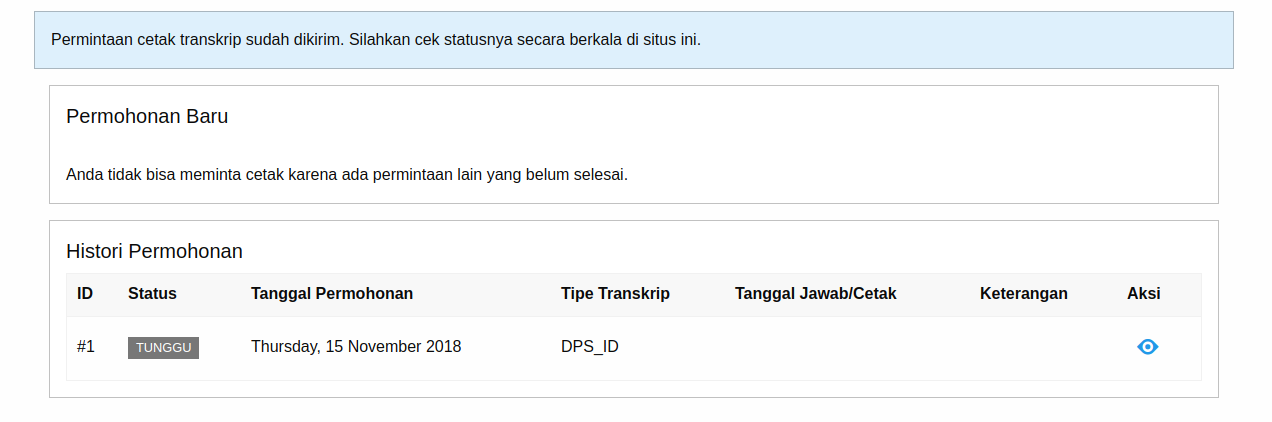
\includegraphics[width=\textwidth]{bluetape-cetak-transkrip-request.png}  
	\caption[Tampilan hasil Request Cetak Transkrip]{Tampilan hasil Request Cetak Transkrip} 
	\label{fig:bluetape-cetak-transkrip-request} 
\end{figure}

\subsubsection{Transkrip \textit{Manage}}
\begin{figure}[H]
	\centering  
	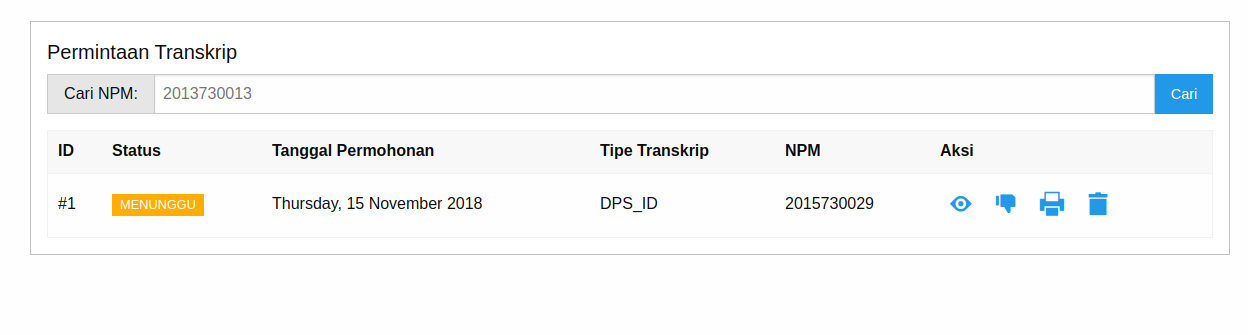
\includegraphics[width=\textwidth]{bluetape-manajemen-transkrip.png}  
	\caption[Tampilan Manajemen Transkrip BlueTape]{Tampilan Manajemen Transkrip BlueTape} 
	\label{fig:bluetape-manajemen-transkrip} 
\end{figure}

\subsubsection{Perubahan Kuliah \textit{Request}}
\begin{figure}[H]
	\centering  
	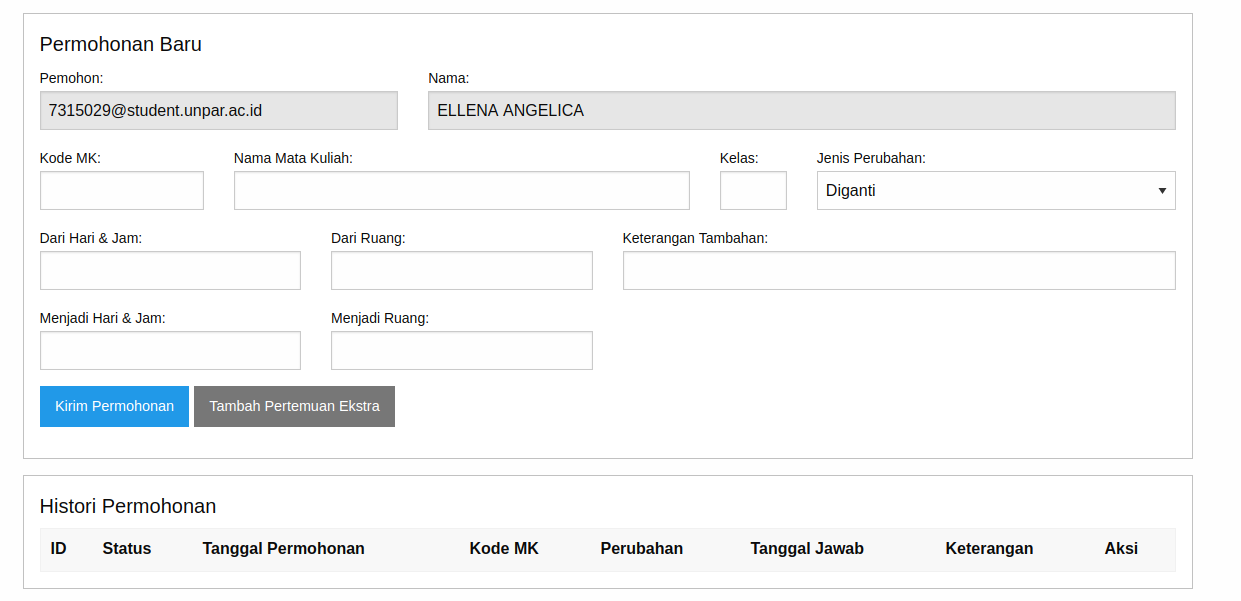
\includegraphics[width=\textwidth]{bluetape-perubahan-kuliah-request.png}  
	\caption[Tampilan request perubahan kuliah]{Tampilan request perubahan kuliah} 
	\label{fig:bluetape-perubahan-kuliah-request} 
\end{figure}

\subsubsection{Perubahan Kuliah \textit{Manage}}
\begin{figure}[H]
	\centering  
	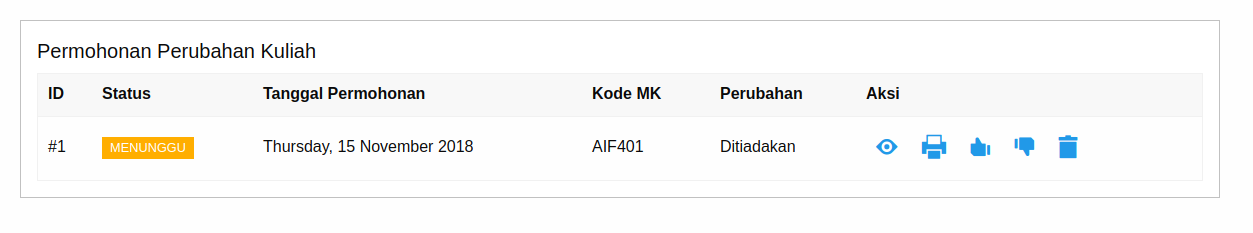
\includegraphics[width=\textwidth]{bluetape-perubahan-kuliah-manajemen.png}  
	\caption[Tampilan manage perubahan kuliah]{Tampilan manage perubahan kuliah} 
	\label{fig:bluetape-perubahan-kuliah-manajemen} 
\end{figure}

\subsubsection{Perekam Jadwal Dosen}
\begin{figure}[H]
	\centering  
	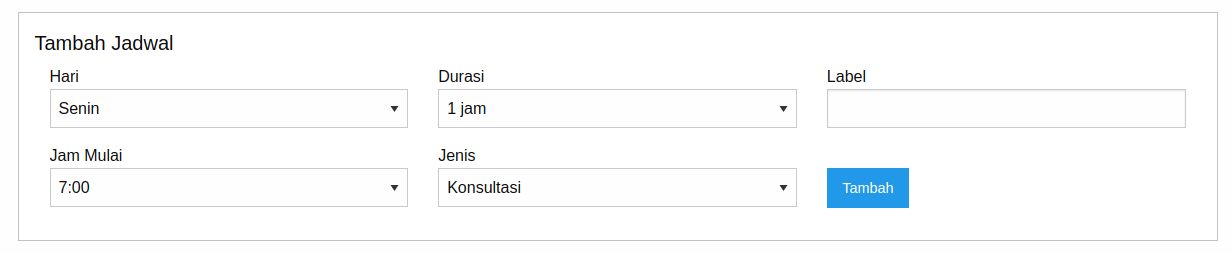
\includegraphics[width=\textwidth]{bluetape-entri-jadwal-dosen-tambah.png}  
	\caption[Tampilan tambah jadwal dosen]{Tampilan tambah jadwal dosen} 
	\label{fig:bluetape-entri-jadwal-dosen-tambah} 
\end{figure}

\begin{figure}[H]
	\centering  
	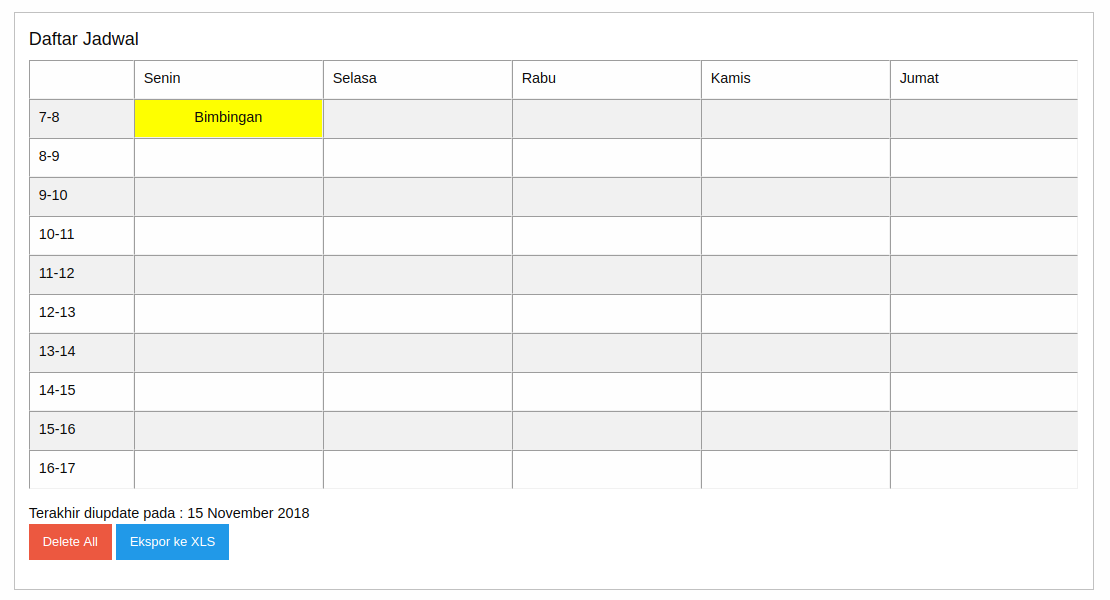
\includegraphics[width=\textwidth]{bluetape-entri-jadwal-dosen-daftar.png}  
	\caption[Tampilan jadwal dosen]{Tampilan jadwal dosen} 
	\label{fig:bluetape-entri-jadwal-dosen-daftar} 
\end{figure}

\begin{figure}[H]
	\centering  
	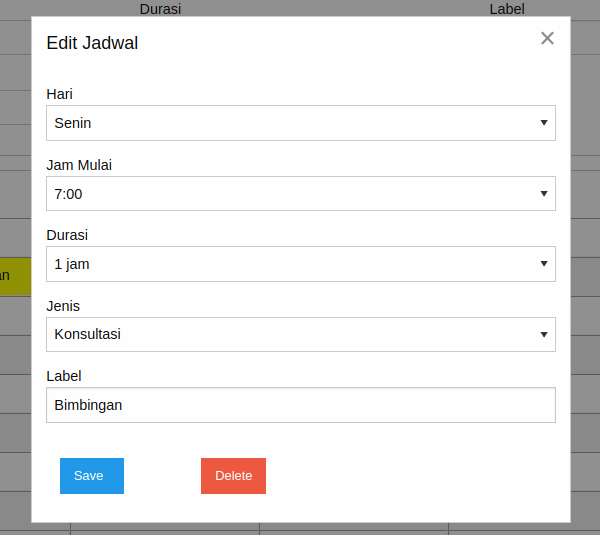
\includegraphics[width=\textwidth]{bluetape-edit-jadwal-dosen.png}  
	\caption[Tampilan edit jadwal dosen]{Tampilan edit jadwal dosen} 
	\label{fig:bluetape-edit-jadwal-dosen} 
\end{figure}

\subsection{Hak Akses}
Hak akses dan nama module diatur pada dokumen \texttt{config/modules.php} yang terletak di dalam direktori \texttt{config}. Hak akses dikelompokkan di dalam kelompok yang disebut \textit{role}. Saat skripsi ini dibuat, hak akses dibagi ke dalam lima \textit{role} : root, mahasiswa.ftis, tu.ftis, staf.unpar, dosen.informatika, dan mahasiswa.informatika. \textit{Role} root berisi daftar alamat email dari pengembang bluetape. \textit{Role} tu.ftis berisi daftar alamat email dari tata usaha ftis. \textit{Role} mahasiswa.ftis berisi daftar alamat email dari mahasiswa ftis. \textit{Role} staf.unpar berisi daftar alamat email dari staf unpar. \textit{Role} dosen.informatika berisi daftar alamat email dari dosen informatika.

Setiap \textit{role} memiliki batasan dalam mengakses module di BlueTape. \textit{Role} root tidak memiliki batasan dan dapat mengakses setiap module yang ada. \textit{Role} tu.ftis hanya dapat mengakses module \texttt{TranskripManage}, dan module \texttt{PerubahanKuliahManage}. \textit{Role} mahasiswa.ftis hanya dapat mengakses module \texttt{TranskripRequest} dan module \texttt{LihatJadwalDosen}. \textit{Role} staf.unpar hanya dapat mengakses module \texttt{PerubahanKuliahRequest}. \texttt{Role} dosen.informatika hanya dapat mengakses module \texttt{EntriJadwalDosen}.

\section{Analisis Heroku}
\label{sec:analisisheroku}
\subsection{BlueTape pada Arsitektur Heroku}
\subsubsection{Dependensi}
BlueTape membutuhkan dependensi tambahan agar perangkat lunak dapat dijalankan. Dependensi tambahan perangkat lunak BlueTape tertera pada dokumen \texttt{composer.json}. Berikut isinya :
\begin{lstlisting}
{
    "require": {
        "google/apiclient": "^1.0",
		"ext-imap": "*",
        "phpoffice/phpexcel": "^1.8",
        "linecorp/line-bot-sdk": "^3.6"
    }
}
\end{lstlisting}

Pada saat skripsi ini ditulis, BlueTape telah memakai dua package : package \texttt{google/apiclient} dan package \texttt{phpoffice/phpexcel}. Package \texttt{google/apiclient} adalah package yang diperlukan untuk autentikasi akun saat masuk ke BlueTape. Sedangkan package \texttt{phpoffice/phpexcel} adalah package yang digunakan untuk menghasilkan dokumen excel. Package yang ditambahkan untuk skripsi ini adalah package \texttt{ext-imap} dan \texttt{line-bot-sdk}. Package \texttt{ext-imap} digunakan untuk mengakses email. Package \texttt{line-bot-sdk} digunakan untuk menghubungkan perangkat lunak dengan layanan yang disediakan oleh LINE.

\subsubsection{Tipe Proses}
BlueTape memiliki satu tipe proses, yaitu tipe proses \texttt{web} dan tipe proses \texttt{release}. Tipe proses \texttt{web} adalah tipe proses yang digunakan untuk menerima arus HTTP eksternal dari router Heroku. Penulis tidak dapat menambahkan tipe proses lain karena itu berarti penulis harus menambah dyno. Penambahan dyno perlu informasi kartu kredit untuk verifikasi akun.

\subsubsection{Procfile}
Procfile adalah dokumen yang menjelaskan Heroku bagian-bagian perangkat lunak yang dapat dieksekusi. Procfile berisi daftar tipe proses beserta cara menjalankannya. BlueTape hanya memiliki satu tipe proses, yaitu tipe proses \texttt{web}. Isi Procfile adalah :
\begin{lstlisting}
web: vendor/bin/heroku-php-apache2 www/
\end{lstlisting}

Maksud dari satu baris Procfile tersebut adalah : untuk menjalankan tipe proses web, heroku harus menjalankan server apache di heroku dan kemudian server menjalankan perangkat lunak web yang ada di direktori \texttt{www}. Perintah \texttt{vendor/bin/heroku-php-apache2} adalah perintah untuk menjalankan server apache di heroku yang ada di package \texttt{heroku-php-apache2}. Package \texttt{heroku-php-apache2} ini otomatis disediakan saat membuat perangkat lunak php di heroku sehingga tidak perlu ditambahkan di composer.json. Perintah \texttt{www/} berguna untuk mengarahkan server apache heroku ke direktori \texttt{www}.

\subsubsection{Slug}
Penulis tidak menambahkan dokumen \texttt{.slugignore} karena tidak diperlukan.

\subsubsection{Buildpack}
Buildpack yang dipakai pada skripsi ini hanya \texttt{heroku/php}. Buildpack ini secara otomatis dipakai oleh Heroku karena BlueTape memakai bahasa PHP.

\subsubsection{Dyno}
Jenis dyno yang dipakai pada skripsi ini adalah free dyno. Jumlah dyno hanya satu. Dyno tersebut merupakan dyno untuk tipe proses \texttt{web}.

\subsubsection{Config Vars}
Config vars yang dipakai di skripsi ini ada banyak : 
\begin{itemize}
\item Config vars untuk informasi database 

\begin{itemize}
\item CI\_DB\_DATABASE 
\item CI\_DB\_HOSTNAME 
\item CI\_DB\_USERNAME
\item CI\_DB\_PASSWORD
\item DATABASE\_URL
\item HEROKU\_POSTGRESQL\_BLUE\_URL
\end{itemize}

\item Config vars untuk autentikasi

\begin{itemize}
\item GOOGLE\_CLIENTID 
\item GOOGLE\_CLIENTSECRET
\end{itemize}

\item Config vars untuk memeriksa email

\begin{itemize}
\item ANNOUNCEMENT\_EMAIL 
\item ANNOUNCEMENT\_PASSWORD
\item HOSTNAME\_INCOMING\_EMAIL
\end{itemize}

\item Config vars untuk informasi dasar situs

\begin{itemize}
\item CI\_BASE\_URL
\end{itemize}

\item Config vars untuk terhubung ke layanan LINE

\begin{itemize}
\item LINE\_BOT\_CHANNEL\_SECRET
\item LINE\_BOT\_CHANNEL\_TOKEN
\end{itemize}

\item Config vars untuk SMTP 

\begin{itemize}
\item SMTP\_HOST
\item SMTP\_PASS
\item SMTP\_PORT
\item SMTP\_USER
\end{itemize}

\end{itemize}

\subsubsection{Region}
Region yang dipakai adalah region default, yaitu United States.

\subsubsection{Stack}
Stack yang dipakai adalah stack yang paling baru, yaitu heroku-18. Stack ini dipilih karena Heroku masa kadaluarsa dukungan untuk stack ini yang paling lama. Alasan lain adalah komputer lokal yang digunakan untuk mengerjakan skripsi ini menggunakan lingkungan yang mirip dengan Heroku, yaitu menggunakan Ubuntu 18.04.

\subsection{Basis Data}
Basis data yang digunakan untuk skripsi ini adalah basis data Heroku Postgres dengan plan hobby-dev. Alasan utama basis data ini digunakan adalah karena penggunaan basis data lain seperti Heroku Redis dan Apache Kafka tidak memungkinkan. Basis data tersebut membutuhkan informasi akun kredit untuk verifikasi akun. Alasan lain adalah basis data ini adalah basis data yang langsung disediakan oleh Heroku.

Sebelumnya BlueTape menggunakan MySQL untuk basis datanya. Proses migrasi dari MySQL ke Heroku Postgres tidak rumit, karena menggunakan fitur Migration dari CodeIgniter. Namun, ada beberapa perubahan pada dokumen Migration. Perubahan-perubahan tersebut adalah :
\begin{itemize}
\item Menyelaraskan nama tabel karena sifat case sensitive pada Postgres
\item Mengubah Replace menjadi Insert dan Update karena Replace tidak didukung oleh Postgres
\item Mengubah tipe data kolom yang sebelumnya menggunakan DATETIME menjadi timestamp
\end{itemize}  

\section{Analisis PHP IMAP}
\label{sec:analisisimap}

\section{Analisis LINE}
\label{sec:analisisline}